\section{Use case 2: Data validation}
Our second use case is about data validation.
Even though the amount of publicly available Linked Open Data (LOD) sets is constantly growing\footnote{See, eg statistics at: \url{http://lod-cloud.net/}.}, 
the diversity of the data employed in applications is mostly very limited:
Only a handful of \rdf data is used frequently~\cite{rietveld2015lod}.
One of the reasons for this is that the datasets' quality and consistency varies significantly,
ranging from expensively curated to relatively low quality data~\cite{zaveri2015quality},
and thus need to be validated carefully before use.

One way to assess data quality is to check them against constraints: 
Users can verify that certain data are fit for their use case,
if the data abide to their requirements.
First approaches to do that were implementations with hard coded validation rules,
such as Whoknows?~\cite{ketterl2011whoknows}.
Lately, attention has been drawn to formalizing RDF quality assessment, more specifically,
formalizing RDF constraints languages, such as Shape Expressions (ShEx)~\cite{shex} or Resource Shapes (ReSh)~\cite{resh}.
This detaches the specification of the constraints from its implementation.

Constraint languages allow users dealing with RDF data and vocabularies
to express, communicate, and test their particular expectations.
Such languages can either be (i) existing frameworks designed for different purposes, eg 
 SPARQL~\cite{hartmann2016,kontokostas2014test},
or OWL~\cite{owlValidation},
or they can be (ii) languages only designed for validation, eg
ShEx~\cite{shex},
ReSh~\cite{resh},
Description Set Profiles (DSP)~\cite{dsp},
or the \wwwc recommended Shapes Constraint Language (SHACL)~\cite{shacl}.
These different languages can be compared
by testing them on commonly supported constraints~\cite{bosch2015rdf,kontokostas2014test},
as conducted by Hartmann (n\'e Bosch) et al~\cite{bosch2015}.

Depending on the users' needs, constraint languages have to be able to cope with very diverse kinds of constraints which 
imply certain \emph{logical requirements}.
Such requirements were investigated by Hartmann et al~\cite{bosch2015} who
identified the Closed World Assumption (CWA) (see also Section~\ref{closedworld}) and the Unique Name Assumption (UNA) -- the assumption that each resource in the domain of discourse 
does have exactly one unique name in the logical language -- as crucial for validation. Since both are not 
supported by many Web Logics, Hartmann et al
 particularly emphasize
the difference between reasoning and validation languages
and favour SPARQL based approaches for validation
which -- if needed -- can be combined with \rdf, \rdf{}S or \owl entailment.
In this section, we take a closer look into these findings from a rule-based perspective:  
We show that neither UNA nor CWA are necessary for validation if a rule-based framework containing predicates 
to compare \uris and literals, and supporting
Scoped Negation as Failure (SNAF) is used. This enables us to --
instead of combining separate, successive systems --
do both \rdf validation \emph{and} reasoning in only one system which acts directly on a constraint language. 
We show the feasibility of this approach by providing an
implementation in Notation3 Logic.
We tackle those constraints
identified by Hartmann et al~\cite{bosch2015} 
which are also covered in RDFUnit \cite{kontokostas2014test}, a validation system which is purely based on SPARQL querying.
We then compare our implementation to the latter. 
Our solution functionally outperforms RDFUnit and our execution time is 
faster for small datasets containing 100.000 triples or less. We can thus perform a task which is often solved by using SPARQL querying with \nthreelogic and obtain comparable results. 

% The remainder of this paper is structured as follows:
% In Section \ref{rw} we discuss related work.
% In Section \ref{cons} we give an overview of common \rdf validation constraints.
% In Section \ref{logic}, we discuss
% how different requirements for \rdf validation are met by rule-based logics.
% Section \ref{n3} explains the details of our proof of concept
% and Section \ref{conc} concludes the paper and provides an outlook 
% for future work.




\subsection{An overview of \rdf validation}\label{rw}

%intro
Below
we first present the state of the art around validation constraint languages.
Then, we will give an overview
of different languages and approaches used for \rdf validation.


%validation: constraints + reasoning
%\rdf validation in general and constraint types
Data quality can be described in many dimensions,
one of them being the intrinsic dimension, namely,
the adherence to a data schema~\cite{zaveri2015quality}.
In the case of \rdf data, this implies adhering to certain constraints.
These have been carefully investigated by several authors (eg Hartmann et al~\cite{hartmann2016}).
%Languages to express constraints
The formulation of (a subset of) these constraints can be done using existing languages (eg OWL)~\cite{owl}, 
the SPARQL Inferencing Notation (SPIN)~\cite{Knublauch2011}, or SPARQL~\cite{sparql})),
or via dedicated languages
(eg Shape Expressions (ShEx)~\cite{shex}, Resource Shapes (ReSh)~\cite{resh}, Description Set Profiles (DSP)~\cite{dsp}, 
or Shapes Constraint Language (SHACL)~\cite{shacl}.
Their execution is either based on reasoning frameworks, or querying frameworks.

On the one hand, Motik et al \cite{motik2007adding} and Sirin and Tau~\cite{sirin2009towards}
propose alternative semantics for OWL
which support the Closed World Assumption,
and are therefore more suited for constraint validation than the original version.
To know which semantics apply,
constraints have to be marked as such.
Using one standard to express both, validation and reasoning,
is a strong point of this approach,
however,  this leads to ambiguity: %as the exact same formula can have different meanings.
%
If the exact same formula can have different meanings, one of the key properties of the Semantics Web -- interoperability -- is in danger.
Another disadvantage of using (modified) OWL as a constraint language
is its limited expressiveness. 
Common constraints such as mathematical operations
or specific checks on language tags
are not covered by OWL~\cite{hartmann2016}.

On the other hand, SPARQL based querying frameworks for validation execution emerged (eg Hartmann \cite{hartmann2016} or Kontokostas et al \cite{kontokostas2014test}).
Where Hartmann proposes SPIN as base language to support validation constraints, Kontokostas introduces a similar but distinct language to SPIN,
more targeted to validation, so-called Data Quality Test Patterns (DQTP). 
DQTPs are generalized  SPARQL queries containing an extra type of variables. In an extra step, these variables are instantiated based on the  RDFS and OWL axioms used
by the data schema and can then be employed for querying. 
As such, the authors assume a closed world semantics for OWL
but in contrast to the approaches mentioned above,
this special semantics cannot be marked in the ontology itself.
They thus change the semantics of the common Web standard OWL.
To also find implicit constraint validation an extra reasoning step could be added,
but this step would then most probably assume the standard semantics of OWL,
further increasing the possibly of experiencing conflicts between the two contradicting versions of the semantics.
Hartmann proposes a dedicated ontology
to express integrity constraints, and as such,
this method does not involve changing existing semantics.
For both, only very limited reasoning can be included directly in the system.
%involving reasoning is not possible without inclusion of a secondary system.



\subsection{\rdf Validation Constraints}\label{cons}


Based on the collaboration of
the W3C \rdf Data Shapes Working Group\footnote{\url{https://www.w3.org/2014/data-shapes/wiki/Main_Page}} and
the DCMI \rdf Application Profiles Task Group\footnote{\url{http://wiki.dublincore.org/index.php/RDF_Application_Profiles}}
with experts from industry, government, and academia,
a set of validation requirements has been defined,
based on which,
81 types of constraints were published,
each of them corresponding to at least one of the validation requirements~\cite{bosch2015rdf}.
This set thus gives a realistic and comprehensive view of what validation systems should support. 


Prior to this, the creators of RDFUnit~\cite{kontokostas2014test} had provided their own set of constraint types they support.
Given the usage of RDFUnit in real-world use cases~\cite{jurion_rdfunit},
this set gives a good overview
of what validation systems should minimally cover.


Table \ref{table:align} shows
the alignment of the 17 types of constraints as supported by RDFUnit
with the relevant constraint types as identified by Hartmann et al~\cite{bosch2015}. 
\sloppy
As can be seen, these types are not mapped one-to-one. 
One constraint from RDFUnit maps to
at least one constraint as identified by Hartmann, 
except for PVT and TRIPLE, which are both not very complex constraints and could thus easily be added to the work of Hartmann et al. 
Here, we mainly focus on these 17 constraints which are all covered by our implementation.
To make the topic of constraint validation more concrete, we discuss the examples (TYPEDEP), (INVFUNC) and (MATCH) in more detail  below
and refer the reader interested  in the other constraint types to the above mentioned sources. 

\begin{table}
\caption{\small Constraints Alignment.
The first column lists the codes as used in RDFUnit;
the second the constraints of Hartmann  following his numbering \cite[appendix]{hartmann2016}; and
the third the description taken from RDFUnit.\normalsize
}
\label{table:align}
\footnotesize
\begin{tabular}{ p{0.2\linewidth} p{0.14\linewidth} p{0.55\linewidth}  } \toprule
\textbf{RDFUnit} & \textbf{Constraint Code} & \textbf{Description} \\ \midrule
 %\hline %\hline 
COMP & A11  &Comparison between two literal values of a resource\\ \midrule
%\hline
MATCH & A20, A21 &A resource's literal value (does not) matches a RegEx\\ \midrule
%\hline
LITRAN & A17, A18 &The literal value of a resource (having a certain type) must (not) be within a specific range\\ \midrule %\hline
TYPEDEP & A4 &Type dependency:  the type of a resource may imply the attribution of another type\\ \midrule %\hline
TYPRODEP & A41 &A resource of specific type should have a certain property\\ \midrule % \hline
PVT & B1 &If a resource has a certain value V assigned via a property P1 that in some way classifies this resource, one can assume the existence of another property P2\\ \midrule %\hline
TRIPLE & B2 &
A resource can be considered erroneous if
there are corresponding hints contained in
the dataset\\ \midrule %\hline
ONELANG & A28 &A literal value has at most one literal for a language\\ \midrule %\hline
RDFS-DOMAIN & A13 &The attribution of a resource's property
(with a certain value) is only valid if the
resource is of a certain type\\ \midrule % \hline
RDFS-RANGE & A14, A15 & The attribution of a resource's property is
only valid if the value is of a certain type\\ \midrule % \hline
RDFS-RANGED & A23 &
The attribution of a resource's property is
only valid if the literal value has a certain
datatype\\ \midrule %\hline
INVFUNC & A2 & Some values assigned to a resource are
considered to be unique for this particular
resource and must not occur in
connection with other resources\\ \midrule % \hline
OWL-CARD & A1, A32--37 & Cardinality restriction on a property\\ \midrule % \hline
OWLDISJC & A70 & Disjoint class constraint\\ \midrule % \hline
OWLDISJP & A69 & Disjoint property constraint\\ \midrule % \hline
OWL-ASYMP & A57 & Asymmetric property constraint\\ \midrule %\hline
OWL-IRREFL & A64 & Irreflexive property constraint \\ \bottomrule
\end{tabular}
\end{table}
\normalsize



\subsection{Features required for Validation}\label{logic}
After having listed the kind of constraints relevant for \rdf validation in the previous section, we will now focus on the suitability of rule-based logics for that task.
Based on the work of Sirin and Tao \cite{sirin2009towards}, and Hartmann et al \cite{bosch2015} who identified the logical requirements constraint 
languages need to fulfil,
we discuss why rule-based logic is a reasonable choice to validate \rdf datasets.




\subsubsection{Reasoning}\label{reasoning}
We start our discussion with reasoning. Hartmann \cite[p. 181]{hartmann2016} points out that performing reasoning in combination with \rdf validation brings several benefits:
constraint violations may be solved, violations which otherwise would stay undetected can be found, and datasets do not need to contain 
redundant data to be accepted by a validation engine. To better understand these benefits, consider the following ontology example:\footnote{As above, the prefix \texttt{rdfs:} 
stands for \url{http://www.w3.org/2000/01/rdf-schema\#}.}
\begin{equation}\label{subc}
 \texttt{:Reseacher rdfs:subClassOf :Person.}
\end{equation}
And the instance:
\begin{equation}\label{Kurt}
 \verb!:Kurt a :Researcher; :name "Kurt01".!
\end{equation}
If we now have a type dependency constraint (TYPEDEP) saying that every instance of the class \texttt{:Researcher} should also be an instance of the class \texttt{:Person}, 
which we test on the data above,
a constraint validation error would be raised since \texttt{:Kurt} is not declared as a \texttt{:Person}. If we perform the same constraint check after reasoning, the triple
\begin{equation}\label{person}
\verb!:Kurt a :Person.!
\end{equation}
would be derived and the constraint violation would be solved. Without the reasoning, Triple~\ref{person}
would need to be inserted into the dataset to solve the constraint,
leading to redundant data. 

To understand how reasoning 
can help to detect implicit constraints, consider another restriction: suppose that we have a constraint stating that a person's name should not contain 
numbers\footnote{This could be expressed by an extended version of MATCH as for example the constraint ``Negative Literal Pattern Matching'' in~\cite{hartmann2016}.}.
Without reasoning, no constraint validation would be detected because even though the \texttt{:name} of \texttt{:Kurt} contains numbers, \texttt{:Kurt} 
would not be detected as an instance of
\texttt{:Person}.


Hartmann's and many other validation approaches thus suggest to first perform a reasoning step and then do an extra validation step via SPARQL querying. 
The advantage of using rule-based reasoning instead is
that validation can take place during the reasoning process \emph{in one single step}. 
Relying on a rule which supports \texttt{rdfs:subClassOf} as  presented 
in~Section~\ref{owlrln3} the aforementioned problem could be detected.
In general, OWL-RL~\cite{OWLRL} can be applied since it is supported by every rule language.
If higher complexity is needed, rule languages with support for existential quantification can be used for OWL QL reasoning.


\subsubsection{Scoped Negation as Failure}
Another aspect which is important for constraint validation is negation.
Hartmann et al claim that the Closed World Assumption is needed to perform validation tasks.
Given that most Web logics assume the Open World Assumption, that would form a barrier for the goal of combining reasoning and validation 
mentioned in the previous section. Luckily, that is not the case.
As constraint validation copes with the local knowledge base,
Scoped Negation as Failure (SNAF) (see also  Section~\ref{closedworld} and for example \cite{damasio2006supporting,kifer2005,polleres2006rules}) is enough.
This is for example supported by FLORA-2~\cite{negflora} or \nthreelogic~\cite{N3Logic}.\footnote{As we will discuss below, SNAF in \nthree is mostly supported by built-in functions. 
As we explicitly excluded these from our discussion in Chapter~\ref{semofn3}, our semantics does not cover SNAF yet. }

In order to understand the idea behind Scoped Negation as Failure,
consider the triples that form Formula~\ref{Kurt}
and suppose that these are the only triples in a 
knowledge base we want to validate. We now want to test the constraint from above that every individual which is declared as a researcher is also declared 
as a person (TYPEDEP). This means our system needs to give a warning if it finds an individual which is declared as a researcher, but not as a person:
\begin{multline}\label{constraint1}
 \forall \texttt{x}: ((\texttt{ x a :Researcher}) \wedge \neg (\texttt{ x a :Person}))\\ \rightarrow (\texttt{:constraint :is :violated.})
\end{multline}
In the form it is stated before, the constraint cannot be tested with the Open World Assumption. 
The knowledge base contains the triple 
\[\texttt{:Kurt a :Researcher.}\]
but not Triple~\ref{person},
but the rule is more general: given its open nature, 
we cannot guarantee that there is no document in the entire Web which declares Triple~\ref{person}.
This changes if we make an addition. Suppose that $\mathcal{K}$ is the
the set of triples
we can derive (either with or without reasoning) from our knowledge base consisting of Formula~\ref{Kurt}. Having $\mathcal{K}$ at our disposal, we can test:
\begin{multline}
 \forall \texttt{x}: ((\texttt{ x a :Researcher})\in \mathcal{K}) \wedge \neg ((\texttt{ x a :Person})\in \mathcal{K}))\\ \rightarrow (\texttt{:constraint :is :violated.})
\end{multline}
The second conjunct is not a simple negation, it is a negation with a certain scope, in this case $\mathcal{K}$. If we added new 
data to our knowledge like for example Triple~\ref{person}, we would have different knowledge $\mathcal{K}'$ for which other statements hold. The truth value of the formula above 
would not be touched since this formula explicitly mentions $\mathcal{K}$. The logic stays monotonic.
%Since we know all triples from $\mathcal{K}$, scoped negation is possible. 
Scoped negation as failure is the kind of negation we actually need in \rdf validation: we do not want to make and
test
statements in the Web in general, we just want to test the information contained in a local file or knowledge base.


\subsubsection{Predicates for Name Comparison}
Next to the Open World Assumption, 
Hartmann et al~\cite{bosch2015}
identify the fact that most Web logics do not base themselves on the Unique Names Assumption (UNA) 
as a barrier for them being used 
for constraint validation. This assumption is for example present in F-Logic \cite{flogic}  and basically states that every element in the domain of discourse
can only have one single name (\uri or Literal in our case).  The reason, why this assumption is in general problematic for the Semantic Web lies in its distributed nature: 
different datasets can -- and actually do -- use different names for the same individual or concept.
For instance, the \uri \texttt{dbpedia:London} refers to the same place in England as 
for example \texttt{dbpedia-nl:London}.\footnote{\texttt{dbpedia} stands for \url{http://dbpedia.org/resource/}, \texttt{dbpedia-nl} for \url{http://nl.dbpedia.org/resource/}.} In this case this fact is even stated in the corresponding ontologies using the 
predicate \texttt{owl:sameAs}.\footnote{As above \texttt{owl} is the prefix for \url{http://www.w3.org/2002/07/owl\#}.}

The impact of the Unique Name Assumption for \rdf validation becomes clear if we take a closer look at OWL's inverse functional property and the related constraint (INVFUNC). 
Let us assume that \texttt{dbo:capital}\footnote{With \texttt{dbo} standing for \url{http://dbpedia.org/ontology/}.} 
is an \texttt{owl:InverseFunctionalProperty} and our knowledge base contains:
\begin{align}\notag
 \texttt{:England dbo:capital :London.}\\\texttt{ :Britain dbo:capital :London.}\label{conflict}
\end{align}
Since \texttt{:England} and \texttt{:Britain} are both stated as having \texttt{:London} as their capital and \texttt{dbo:capital} is an inverse functional property,
an OWL reasoner would derive  
\begin{equation}
 \texttt{:England  owl:sameAs :Britain.}
\end{equation}
Such a derivation cannot be made if the Unique Name Assumption is valid, since the former explicitly excludes this possibility. 

The constraint (INVFUNC) is related to the OWL concept above, but it is slightly different: while OWL's inverse functional property refers to the elements of the domain of
discourse denoted by the name, the validation constraint (INVFUNC) refers to the representation itself. Formula~\ref{conflict} thus violates the constraint. 
Even if our logic does not 
follow the Unique Name Assumption, this violation can be detected if the logic offers predicates to compare names.
In \nthreelogic,
\texttt{log:equalTo} and \texttt{log:notEqualTo}\footnote{\url{https://www.w3.org/2000/10/swap/doc/CwmBuiltins}.} are such predicates: in contrast to
\texttt{owl:sameAs} and \texttt{owl:differentFrom}, they do not compare the resources they denote, but their representation. 
The idea to support these kinds of
predicates is very common. So does, for example,
the Rule Interchange Format (RIF) cover several functions which can handle \uris and strings, 
as we will discuss in the next subsection.
 






\subsubsection{RIF Built-ins}\label{bisec}
In the previous subsection we indicated that a special predicate of a logic,
in this case \texttt{log:notEqualTo}, can be used to do \uri comparisons
and thereby support a concept which would otherwise be difficult to express. 
Such built-in functions are widely spread in rule-based logics
and play an important role in \rdf validation which very often deals with string comparisons, calculations or operations on \uri level.
While it normally depends on the designers of a logic which features are supported, there are also common standards. 

The most important standard for rules in the Semantic Web is RIF
%One of them is the Rule Interchange Format (RIF) \cite{rif}
%whose aim it is to provide a formalism
which was developed to exchange rules in the Web. 
Being the result of a \wwwc working group consisting of developers and users 
of different rule-based languages, RIF can also be understood as a reference for the most common features rule based logics might have. 
This makes the list of predicates~\cite{rifpredicates} supported by the different RIF dialects particularly interesting for our analysis. 
%\todo{AD: The next sentence is really loooong!}
And it is indeed the case that by
only using RIF predicates many of the constraints listed in Section \ref{cons} can already be checked: 
negative pattern matching (MATCH) can be implemented by using the predicate 
\texttt{pred:matches},\footnote{
\texttt{PREFIX pred:} \url{<http://www.w3.org/2007/rif-builtin-predicate\#>}.} 
the handling of language tags as required for the constraint ONELANG can be done using \texttt{func:lang-from-PlainLiteral},\footnote{\texttt{PREFIX func:}
\url{<http://www.w3.org/2007/rif-builtin-function\#>}}
 and for the comparison of literal values (COMP) there are several predicates to compare strings, numbers or dates.


To illustrate  how powerful RIF is when it comes to string validation, we take a closer look at the predicate \texttt{log:notEqualTo} from the previous section. 
In the example above it is used to compare two \uri representations and succeeds if these these two are different. To refer to a \uri value, RIF provides the predicate 
\texttt{pred:iri-string} which converts a \uri to a string and and vice versa. In \nthree notation\footnote{The EYE reasoner supports RIF predicates.
These need to be used in \nthree syntax.} 
that could be expressed by:
%\small
\begin{multline}
\texttt{(:England "http://exmpl.com/England")}\\\texttt{ pred:iri-string true.}
\end{multline}
%\normalsize
To compare the newly generated strings, the function \texttt{func:compare} can be used. This function takes two string values as input,
and returns -1 if the first string 
is smaller
than the second one regarding a string order, 0 if the two strings are the same, and 1 if the second is smaller than the first. The example above gives:
\begin{multline}
 \texttt{("http://exmpl.com/Britain"}\\\texttt{ "http://exmpl.com/England")}\\ \texttt{func:compare -1.}
\end{multline}
\sloppy
To enable a rule to detect whether the two \uri names are equal, one additional function is needed: the reasoner has to detect whether the result of the comparison
is not equal to zero. 
That can be checked using the predicate \texttt{pred:numeric-not-equal} which is the RIF version of $\neq$ for numeric values. In the present case the output 
of the comparison would be 
\texttt{true} since $0\neq 1$, a rule checking for the name equality of \texttt{:England} and \texttt{:Britain} using the three predicates would therefore be triggered.

Even though we needed three RIF predicates to express one \nthree predicate, the previous example showed how powerful built-ins in general -- but also the very common RIF predicates
in particular -- are. Whether a rule based Web logic is suited for \rdf validation highly depends on its built-ins. If it supports all RIF predicates, this can be seen as a strong
indication that it is expressive enough.


\subsection{Validation with \nthreelogic}\label{n3}
In the previous section we analysed the requirements
on a rule-based Web logic to be able to combine validation and reasoning:
it should support scoped 
negation as failure, it should provide predicates to compare different \uris and strings, and its built-in functions should be powerful enough to, inter alia, 
access language tags
and do string comparison as they are supported by RIF.
\nthreelogic as it is implemented in the EYE reasoner \cite{eyepaper} fulfils all these conditions. 
With that logic, we were able to implement rules for all the constraints listed in Section~\ref{cons}, and thus 
provide similar functionality as RDFUnit using rule-based Web logics.
Below we discuss the
details of this implementation. % starting by providing more information about \nthreelogic and EYE. 
The rules for our implementation can be accessed at \url{https://github.com/IDLabResearch/data-validation}. 



% \subsubsection{\nthreelogic}\label{n3syn}
% \nthreelogic was introduced in 2008 by Tim Berners-Lee et al \cite{N3Logic} and is an extension of \rdf:
% All \rdf turtle triples are also valid in \nthree. 
% As in \rdf, blanknodes are understood as existentially quantified variables and the co-occurrence of two triples as in Formula~\ref{conflict} 
% is understood as their conjunction. \nthree furthermore supports universally quantified variables. These are indicated by a leading question mark \texttt{?}. 
% \begin{equation}
%  \texttt{?x :likes :IceCream.}
% \end{equation}
% stands for \textit{``Everyone likes ice cream.''},  or in first order logic
% \[\forall x: \text{likes}(x, \text{ice-cream})\]
% Rules are written using curly brackets \texttt{\{~\}} and the implication symbol \texttt{=>}. The \texttt{rdfs:subClassOf} 
% relation from Formula~\ref{subc} can be expressed as:
% \begin{equation}\label{rulescl}
%  \texttt{\{?x a :Researcher\} => \{?x a :Person\}.}
% \end{equation}
% Applied on Formula~\ref{Kurt} the rule results in Formula~\ref{person}. 
% More details about syntax and semantics of \nthree can be found in our previous paper \cite{arndt_ruleml_2015}.
% 
% There are several reasoners supporting \nthree:
% FuXi \cite{fuxi} is a forward-chaining production system for Notation3 whose reasoning is based on the RETE algorithm. 
% The forward-chaining cwm \cite{cwm} reasoner 
% is a general-purpose data processing tool which can be used for querying, checking, transforming 
% and filtering information.
% EYE \cite{eyepaper} is a reasoner enhanced with Euler path detection. 
% It supports 
% backward and 
% forward 
% reasoning and also a user-defined mixture of both. 
% Amongst its 
% numerous features are the option to skolemise blank nodes
% and  the possibility to produce and reuse proofs for further reasoning. 
% The reason why we use EYE in our implementation is its generous support for built-ins\footnote{\url{http://eulersharp.sourceforge.net/2003/03swap/eye-builtins.html}}: 
% next to \nthree's native built-ins\footnote{\url{https://www.w3.org/2000/10/swap/doc/CwmBuiltins}}, 
% RIF, but also several other functions and concepts are implemented. 


\subsubsection{Expressing Constraints}


\begin{lstlisting}[
  float=t,
  caption={Example inverse functional property constraint: No city can be the capital of two countries. },
  label=example2]
§\textcolor{gray}{@prefix rdfcv: \url{<http://www.dr-thomashartmann.de/phd-thesis/rdf-validation/vocabularies/rdf-constraints-vocabulary\#>}.}§
§\textcolor{gray}{@prefix : <http://example.org/ex\#>.}§
§\textcolor{gray}{@prefix dbo: 	<http://dbpedia.org/ontology/> .}§

:example_constraint a rdfcv:SimpleConstraint ;
  :constraintType :InverseFunctionalProperties ;
  rdfcv:constrainingElement :inverse-functional-properties ;
  rdfcv:leftProperties ( dbo:capital ) ;
  rdfcv:contextClass  dbo:Country .
\end{lstlisting}

Before we can detect violations of constraints using \nthree logic,
these constraints first need to be stated.
This could either be done by directly expressing them in 
rules -- and thereby creating
a new constraint language next to the ones presented in Section~\ref{rw} -- or on top of existing \rdf-based conventions. 
%The first option would require a certain level of knowledge of \nthree and its builtins---for example \nthree's way to express scoped negation as failure---
%While the first option would require a deeper knowledge of \nthree and its built-in functions, the second option just expects the user to know \rdf and  
We opt for the latter and base our present implementation on the work of Hartmann \cite[p.167 ff]{hartmann2016}:
in his PhD thesis, Hartmann presents a lightweight vocabulary to describe any constraint, 
the RDF Constraints Vocabulary (RDF-CV)\footnote{\url{https://github.com/boschthomas/RDF-Constraints-Vocabulary}}. The reason why we chose that vocabulary over 
the upcoming standard
SHACL is its expressiveness. We aim to tackle the 81 constraints identified by Hartmann which are not all expressible in SHACL 
or any other of the constraint languages
mentioned in Section~\ref{rw} \cite[p.52, appendix]{hartmann2016}. As will be shown in the following section, it is not difficult to adopt the rules to different 
constraint languages as long as they are based on \rdf and as such valid \nthree expressions.

RDF-CV supports the concept of so called \emph{simple constraints} which are all the constraints expressible by the means of the vocabulary, in particular 
the ones mentioned in Section~\ref{cons}. Each simple constraint has a constraining element. Where applicable, the names of these elements are inspired by their related 
DL names, but the constraining element can also be for example the name of a SPARQL function. In some cases, the same constraint type 
can be marked by different constraining elements as for example the constraint COMP whose constraining element is the relation 
used to compare values 
(eg the usual numerical orders: $<,>,\leq$, and $\geq$) or there can be different constraint types sharing the same constraining element.
To be sure that cases like this do not cause any ambiguity we additionally assign a \emph{constraint type} to every constraint. 
The names of these types follow the names used by Hartmann~\cite[appendix]{hartmann2016}. 
The TYPEDEP constraint from Section~\ref{reasoning} is for example of constraint type \texttt{:Subsumption}.

In addition to constraining element and constraint type, there are several predicates to assign the constraints to individuals and classes: \emph{context class}, 
\emph{classes}, 
\emph{leftProperties}, 
\emph{rightProperties}, and \emph{constraining values}.
The \emph{context class} of a constraint fixes the set of individuals for which a constraint must hold. For the subsumption constraint mentioned above, that would be 
the class \texttt{:Researcher}, the constraint talks about \emph{every} individual labelled as \emph{researcher}. 
There could be other classes involved. In our subsumption example that is the superclass the  
individuals should belong to, \texttt{:Person}. Every researcher should also be labelled as \emph{person}. %The whole subsumption example is displayed in Listing~\ref{subcc}. 
Since these kinds of properties can be multiple, 
they are given in a
list. How and if the predicate  \emph{classes} is used depends on the constraint.
The predicates \emph{leftProperties} and \emph{rightProperties} are used to do similar statements about properties. The constraint INVFUNC as displayed in 
Listing~\ref{example2} makes for example use of it to 
relate the constraint specified to the predicate it is valid for. The objects of the predicates \emph{leftProperties} and \emph{rightProperties} are lists. The predicate 
\emph{constraining value}
 is used for the predicates where a literal value is needed to further specify a constraint. An example for such a constraint is MATCH as described in Section~\ref{reasoning}. To 
 express, that a name should not contain numbers, the predicate \emph{constraining value} connects the constraint to the string pattern,
 \texttt{"[1-9]"} in the present case. 



\subsubsection{Constraint Rules}\label{rules}
\begin{lstlisting}[
  float=t,
  caption={Rule for inverse functional property (INVFUNC). The predicate \texttt{log:notEqualTo} compares the resources based on their URI and thereby supports 
  the Unique Name Assumption. },
  label=invfunc]
§\textcolor{gray}{@prefix rdfcv: \url{<http://www.dr-thomashartmann.de/phd-thesis/rdf-validation/vocabularies/rdf-constraints-vocabulary\#>} .}§
§\textcolor{gray}{@prefix : <http://example.org/ex\#> .}§
§\textcolor{gray}{@prefix list: <http://www.w3.org/2000/10/swap/list\#>.}§
§\textcolor{gray}{@prefix log: <http://www.w3.org/2000/10/swap/log\#> .}§

{
?constraint a rdfcv:SimpleConstraint;
  :constraintType :InverseFunctionalProperties;
  rdfcv:constrainingElement :inverse-functional-properties;
  rdfcv:leftProperties ?list;
  rdfcv:contextClass  ?Class.
  
?object a ?Class.
?property list:in ?list.
?x1 ?property ?object.
?x2 ?property ?object.
?x1 log:notEqualTo ?x2
}
=>
{
[] a :constraintViolation;
    :violatedConstraint ?constraint.
}.
\end{lstlisting}


Having seen in the last section one possible way to describe constraints on \rdf datasets, this section explains how these descriptions can be used. We employ rules
which take the expressed constraints and the \rdf dataset to be tested into account and generate triples indicating constraint validations, if present. 
We illustrate that by an example: In  Listing~\ref{invfunc} we provide a rule handling the constraint INVFUNC. Lines 7--11 contain the details of the constraint. The rule
applies for simple constraints of the type \emph{inverse functional properties} for which a context class \texttt{?Class} and a list \texttt{?list} of left properties 
is specified.
This part of the rule's antecedence unifies with the constraint given in Listing \ref{example2}. Lines 13--18 describe which situation in the tested data causes 
a constraint violation: for an \texttt{?object} which is an instance of \texttt{?Class}, there are two subjects, \texttt{?x1} and \texttt{?x2}, defined 
which are both connected 
to \texttt{?object} via \texttt{?property}. This \texttt{?property} is an element of \texttt{?list},
and the names, ie the \uri- or string-representations, of \texttt{?x1} and \texttt{?x} differ. The latter is expressed using the predicate
\texttt{log:notEqualTo}\footnote{As explained in Section~\ref{bisec} 
there are alternative ways to express the predicate \texttt{log:notEqualTo} in \nthree, the antecedence of the entire rule could also be expressed only using RIF predicates.} 
(Line 18). Together with Listing~\ref{example2} that violation is thus detected if two different resource names 
for resources of the class \texttt{dbo:Country} are connected via the predicate \texttt{dbo:capital} to the same object. Assuming that \texttt{:Britain} and \texttt{:England}
are both instances of the class \texttt{dbo:Country}, the triples in Formula~\ref{conflict} lead to the violation:
\begin{multline}
 \texttt{\_:x a :violaton;}\\\texttt{ :violatedConstraint :example\_constraint.}
\end{multline}
The example relies on descriptions following the vocabulary Hartmann suggests, but our approach can easily be adapted for 
other constraint vocabularies whose syntax is based on \rdf. We only need rules to translate from one concept to another. Similarly, we can generate constraints we want to test later on 
using rules, this is what we explain below.

\subsubsection{Generating constraint descriptions}
\begin{lstlisting}[
  float=t,
  caption={Example constraint (TYPEDEP). This constraint tests whether the derivations implied by Formula~\ref{subc} have been produced. },
  label=ty]
§\textcolor{gray}{@prefix rdfcv: \url{<http://www.dr-thomashartmann.de/phd-thesis/rdf-validation/vocabularies/rdf-constraints-vocabulary\#>} .}§
§\textcolor{gray}{@prefix : <http://example.org/ex\#> .}§

_:example_constraint_2 a rdfcv:SimpleConstraint ;
  :constraintType :Subsumption ;
  rdfcv:constrainingElement :sub-class ;
  rdfcv:contextClass  :Researcher;
  rdfcv:classes :Person .
\end{lstlisting}
One use case for constraint testing -- apart from simple quality assurance -- is to test whether a reasoner or any other application which automatically 
adds triples to a triple store works properly. 
%In these cases, the reasoning and the testing should be performed by two independent systems.
To better understand this special case and how this can be approached using \nthree, we come back to our reasoning example above. Via subclass reasoning an 
\owl DL reasoner should derive Formula~\ref{person} from the  TBox-triple~\ref{subc} and the ABox-formula~\ref{Kurt}. % and  

Above, we discussed, how this reasoning can also be performed by using \nthree. Here, instead of applying this reasoning, we want to test, whether the data set 
which is produced by another system contains Formula~\ref{person} given that the Formulas~\ref{subc} and \ref{Kurt} are also present. 
To do so, we can declare a TYPEDEP constraint as displayed in Listing~\ref{ty}. But in this case -- testing the output of a reasoner -- we already know that we want to perform a similar test
for all \texttt{rdfs:subClassOf}-declarations in our ontology's TBox. 
We can thus use a rule to automatically produce the constraint descriptions. We display such a rule in Listing~\ref{tyrule}.
Applied on Formula~\ref{subc} we get an instance of The formula displayed in Listing~\ref{ty}. We can write similar rules for other ontology concepts and we can translate other constraint 
vocabularies to RDF-CV. 

This translation can be performed in one single reasoning run together with the validation. By using translation or generation rules together with validation rules we
which can be selected according to the user's need we have a very strong and at the same time very flexible system.

% 
% Other implementations we are aware of (in particular RDFUnit), perform similar translation steps as the one we describe above. In contrast to our approach, these translation steps 
% often need to be performed prior to the constraint testing while in our implementation we can generate or translate constraint descriptions in the same reasoning run the constraints are tested.

\begin{lstlisting}[
  float=t,
  caption={Rule producing a (TYPEDEP) constraint from an \texttt{rdfs:subClassOf} declaration. Such rules can be used to test reasoners. },
  label=tyrule]
§\textcolor{gray}{@prefix rdfcv: \url{<http://www.dr-thomashartmann.de/phd-thesis/rdf-validation/vocabularies/rdf-constraints-vocabulary\#>} .}§
§\textcolor{gray}{@prefix : <http://example.org/ex\#> .}§
§\textcolor{gray}{@prefix rdfs: <http://www.w3.org/2000/01/rdf-schema\#>.}§

{
?x rdfs:subClassOf ?y
}
=>
{
_:constraint a rdfcv:SimpleConstraint ;
  :constraintType :Subsumption ;
  rdfcv:constrainingElement :sub-class ;
  rdfcv:contextClass  ?x;
  rdfcv:classes ?y .
}.
\end{lstlisting}

% As an example we  If we for example want to test, whether all occurrences of the term \texttt{rdfs:subclassOf} occurring in an \owl DL ontology were 
% interpreted correctly by a reasoner when producing the deductive closure of the TBox and the ABox of an ontology, ie whether 
% %  Similarly, we can generate constraints using rules in case
% % we want to test certain details based on existing patterns in an ontology. 
% % This is what we explain
% % below.
% To better understand the latter, we come back to the constraint type \emph{inverse functional properties} we discussed above. We already said that stating 
% such a type of constraint is not the same as using
% %All  we need is a consistent way to express constraints in \rdf. 
% the \owl concept \texttt{owl:InverseFunctionalProperty} in an ontology: % and assume that in the context it is used it is meant as a constraint 
% While the latter can be understood in an declarative manner -- is 
% 
% 
% 
% 
% Next to the freedom of our \nthree  implementation of basing our rules on any constraint vocabulary which is syntactically based on \rdf we can also connect 
% 
% Explain: once we fixed a constaint vocabbulary, we do not need to stick to it, we can write additional rules to map from one vocabulary to another. If we for example 
% follow the different approches based on \owl which often change the fixed semantics of \owl we can 

\subsection{Evaluation}
In the previous section we described how we can use \nthree to perform constraint testing and -- if necessary -- combine these tests with constraint generation or ontology reasoning.
We call our implementation \enquote{Validatrr}: a validator using rule-based reasoning. Validatrr makes use of the EYE reasoner.
To be able to compare our implementation with existing approaches, a Node.js JavaScript framework was created
to discover and retrieve vocabularies and ontologies, manage command line arguments and run tests.
This framework is available at \url{https://github.com/IDLabResearch/validatrr}.

For our evaluation, we compare Validatrr with an implementation based on SPARQL querying: RDFUnit~\cite{kontokostas2014test}. 
We want to know how Validatrr performs in terms of accuracy -- that is, do they correctly detect the same constraint violations -- and execution times 
compared to the latter. Below, we discuss both aspects separately.

\subsubsection{Accuracy}
\begin{table}
	\centering
	\caption{\small Comparing RDFUnit to Validatrr using different sets of inferencing steps ($\emptyset$ and $\upsilon$). %, and $\rho$).
		Validatrr finds more violations given the same set of inferencing steps. % and the set of inferencing steps used impacts the result.
		Test cases where Validatrr outperforms RDFUnit are starred. Rows where Validatrr and RDFUnit differ are marked grey.}
	\label{table:unit-test}
	\footnotesize
	\begin{tabular}{rccc} \toprule
		%\hline 
		\bf Test Case & \multicolumn{3}{c}{\textbf{\# found violations}} \\
		& \makecell{RDFUnit} & \multicolumn{2}{c}{Validatrr} \\
		& $\upsilon$ & $\emptyset$ & $\upsilon$ \\
		\hline
		{{\scshape invfunc}\_correct} & 0 & 0 & 0  \\ 
		\rowcolor{lightergrey} \textit{{\scshape invfunc}\_wrong} & 2 & 0 & 2 \\ 
		{{\scshape owlcardt}\_correct} & 0 & 0 & 0  \\ 
		{{\scshape owlcardt}\_wrong\_exact} & 6 & 6 & 6 \\ 
		{{\scshape owlcardt}\_wrong\_max} & 2 & 2 & 2  \\ 
		{{\scshape owlcardt}\_wrong\_min} & 2 & 2 & 2  \\ 
		{{\scshape owldisjc}\_correct} & 0 & 0 & 0  \\ 
		\rowcolor{lightergrey} \textit{{\scshape owldisjc}\_wrong} & 6 & 2 & 6  \\ 
		{{\scshape owlqcardt}\_correct} & 0 & 0 & 0  \\ 
		{{\scshape owlqcardt}\_wrong\_exact} & 6 & 6 & 6 \\ 
		{{\scshape owlqcardt}\_wrong\_max} & 2 & 2 & 2  \\ 
		{{\scshape owlqcardt}\_wrong\_min} & 2 & 2 & 2  \\ 
		{{\scshape rdflangstring}\_correct} & 0 & 0 & 0  \\ 
		{\scshape rdflangstring}\_wrong & 2 & 2 & 2 \\ 
		\rowcolor{lightergrey} \textit{{\scshape rdfsrange-miss}\_wrong*} & 1 & 3 & 3  \\ 
		{{\scshape rdfsranged}\_correct} & 0 & 0 & 0  \\ 
		\rowcolor{lightergrey} \textit{{\scshape rdfsranged}\_wrong*} & 2 & 3 & 3  \\ 
		\rowcolor{lightergrey} \textit{{\scshape rdfsrange}\_correct*} & 0 & 5 & 4  \\ 
		\rowcolor{lightergrey} \textit{{\scshape rdfsrange}\_wrong*} & 1 & 3 & 3  \\ 
		{\scshape rdfsrang\_lit}\_correct & 0 & 0 & 0 \\ 
		{\scshape rdfsrang\_lit}\_wrong & 3 & 3 & 3  \\
		\bottomrule 
	\end{tabular} 
	%\medskip
\end{table}
\normalsize
To test for both implementations whether they correctly detect all constraint violations they are supposed to find when provided with a set of constraint descriptions and
files to check for those we used the unit tests written for RDFUnit which we directly
took from the RDFUnit repository\footnote{\url{https://github.com/AKSW/RDFUnit/tree/master/rdfunit-core/src/test/resources/org/aksw/rdfunit/validate/data}}.
As mentioned above, constraints in RDFUnit are expressed using SPARQL patterns, so-called DQPTs. 
We translated these DQTPs to RDF-CV according to the mapping given in Table~\ref{table:align}.
Apart from this, there was no difference in the input sets of both validation systems and 
we used all test patterns available\footnote{For a detailed description of these test patterns we refer to
the original publication of RDFUnit~\cite{kontokostas2014test}.}.
RDFUnit furthermore uses a custom set of inference rules: each resource is an \texttt{rdfs:Resource} and the construct \texttt{rdfs:subclassOf} is understood according to its meaning defined in 
RDFS semantics~\cite{RDFSemantics}. We call this set of rules $\upsilon$. 

In Table~\ref{table:unit-test} we display the results of our tests using RDFUnit, Validatrr without extra reasoning  ($\emptyset$) and Validatrr using the rules $\upsilon$.
We list the name of the test cases together with the number of constraint violations each implementation found. 
% We clearly see that when applying the same reasoning as RDFUnit, Validatrr
% finds the same or a higher number of constraint violations as RDFUnit.
We marked each test case for which Validatrr finds more violations than RDFUnit with a star. These are the cases 
\textit{{\scshape rdfsrange-miss}\_wrong}, \textit{{\scshape rdfsranged}\_wrong}, \textit{{\scshape rdfsrange}\_correct} and \textit{{\scshape rdfsrange}\_wrong}.
All these cases contain the restriction type \emph{multiple range} which is not yet supported by RDFUnit: when the predicate \texttt{:multRanges} is used, 
each resource linked as an object to that predicate should be classified into multiple classes. For all other cases the number of encountered constraints is the same for both
implementations when applying the same set of inference rules. Our approach thus outperforms RDFUnit.




\subsubsection{Performance}
After comparing both implementations in terms of accuracy, we now want to have a closer look at their execution time. To test this, we again follow 
RDFUnit's original evaluation method. RDFUnit derives constraints from the existing schemas FOAF, GeoSPARQL, OWL, DC terms, SKOS, and Prov-O. 
The idea behind that is similar as we discussed it above when we showed how a rule can be used to generate a constraint from the concept \texttt{rdfs:subClassOf}. RDFUnit uses a step 
to first generate DQPTs based on the concepts found in an ontology while we use extra rules.

For our concrete test 
we used graphs following these  schemas.
At most ten different \rdf graphs --~per schema, per \rdf graph size~-- were downloaded,
by querying LODLaundromat's SPARQL endpoint~\cite{beek2014lod}.
In total we downloaded
300~%
graphs with sizes ranging from ten to one~million triples. For each of these datasets constraints were created according to the schema they were following and then tested.
The tests were executed on a  machine consisting of 24 cores (Intel Xeon CPU E5-2620 v3 @ 2.40GHz) and 128GB RAM.
All evaluations were performed using untampered docker images for both approaches to maintain reproducibility,
the different tests were orchestrated using custom scripts.
All timings include the docker images' initialization time.
The data is available at \url{https://github.com/IDLabResearch/validation-benchmark/tree/master/data/validation-journal}.

In Figure~\ref{fig:eval-size} we show the results of our tests: we plotted the median execution time of all schemas against the \rdf graph size for both approaches.
We clearly see that for small datasets containing less than 100,000 triples our solution is faster than RDFUnit. 

% The median execution time across all schemas is plotted against \rdf graph size per approach
% in a log-log scale
% (see \cref{fig:eval-size}).
% To make sure we can combine execution times across schemas,
% we tested the null hypothesis that no significant difference in execution time was found between schemas,
% by performing an ANOVA statistical test with single factor ``used schema'' for measurement variable
% ``execution time per triple'',
% executed pairwise for all used schemas.
% The null hypothesis with $\alpha = 0.05$ was accepted
% for every pair.
% %Processing times larger than two minutes
% %are not kept in the plot but denoted with a red cross.
% The number of found violations are not plotted,
% as statistical analysis shows no large correlation
% between execution time and number of found violations,
% neither for Validatrr or RDFUnit ($-0.0203$ and $0.0458$, respectively).

% Note that our rules act directly on constraint descriptions and \rdf datasets: while the SPARQL based approaches \cite{hartmann2016,kontokostas2014test} mentioned 
% in Section~\ref{rw} rely on an extra mapping step
% to instantiate the search patterns. If reasoning needs to be included into the data validation, a rule based system can do reasoning, mapping and constraint validation 
% in one single step  where other systems need to perform three.

\begin{figure}[t]
    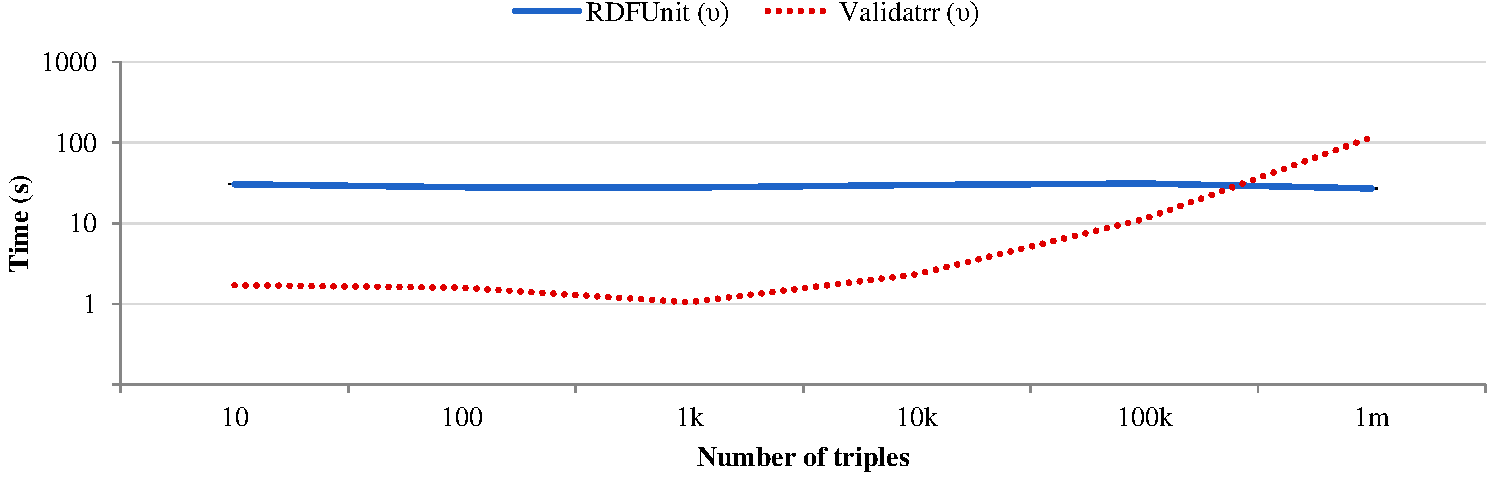
\includegraphics[width=\linewidth]{eval_size.pdf}
\caption{Validatrr's execution speed (dotted line) is up to an order of magnitude faster than RDFUnits's (solid line) when the number of triples per \rdf graph is below 100,000 triples.}
	\label{fig:eval-size}
\end{figure}


\subsection{Discussion}\label{conc}
Above we compared our rule-based \rdf validation system Validatrr with another state-of-the art system providing that service. The difference between Validatrr and RDFUnit 
lies in the technologies used: RDFUnit first instantiates SPARQL patterns (DQPTs) using a programming script and then applies these queries 
while Validatrr uses \nthreelogic for both of these steps. %We saw that our implementation can support all constraint types which are covered by RDFUnit. 
This quality of a unifying logic -- supporting constraint generation and testing at the same time -- made that our approach performed faster on small datasets. Similarly,
more advanced reasoning as for example
discussed in Section~\ref{owlrln3} could be added.
Validatrr was furthermore more accurate on the test cases we 
performed and could correctly spot more constraint violations.

If we come back to our initial question ``Can \nthree solve the same practical tasks as SPARQL querying with a comparable performance?'' 
we can again give a positive answer for our use case: RDF validation can 
be performed by using \nthree reasoning and for smaller datasets \nthree outperforms the solution using SPARQL. 
But we need again to be careful with that answer: 
Our positive results could be achieved because \nthree as implemented in the EYE reasoner 
offers three important features which are crucial for data validation: It supports SNAF, it provides predicates to compare names (and thereby makes an UNA unnecessary), and it
has powerful built-ins to for example, 
do string comparisons or access language tags. Not all of these features are covered in the original specification 
about \nthreelogic~\cite{Notation3,N3Logic} and it depends on the discussion within the community\footnote{See also: \url{https://github.com/w3c/N3/issues/11}.} whether or not these
become an official part of that logic. But if this is the case, \nthree is powerful enough to support all constraint types which are covered by RDFUnit.


% we discussed the possibility to use a rule-based logic to perform \rdf validation.
% We identified the support of SNAF, predicates for name comparison and powerful built-ins as the key components a logic should have to be able to fulfil this task. 
% As \nthree fulfils all these requirements, we implemented Validatrr, a rule-based system to perform \rdf validation. By using 
% 
% 
% Above we discussed the different requirements a rule based Web logic needs to fulfil to be suitable for \rdf validation:
% it should support Scoped Negation as Failure, it should provide predicates for name comparison, and its built-ins should be powerful enough to, for example, 
% do string comparisons or access language tags. 
% 
% The main reason for this difference in performance is that we use the same technology -- \nthreelogic as a potentially unifying logic -- which can generate constraints 
% from existing schemas and test data 
% for validation of these constraints as opposed to RDFUnit where these two tasks need to be executed by two different technologies -- a custom system to instantiate DQTPs and 
% SPARQL-querying.


% 
%  Together with the capability to meet its primary purpose, Web reasoning, such a Web logic is
% a strong alternative to the common approach of either combining reasoning and validation in two different steps, for example by first performing OWL reasoning and 
% then executing SPARQL queries on top of the result as done by Hartmann \cite{hartmann2016}, or only executing SPARQL queries and thereby ignoring possible 
% implicit constraint violations
% as done in RDFUnit~\cite{kontokostas2014test}. Rule based Web logics fulfilling the requirements still provide the same expressivity as SPARQL with the additional advantage
% of supporting reasoning. Validation and reasoning can thus be done by \emph{one single system} in \emph{one single step}. 
% %
% The practical feasibility of this approach has been shown by providing a proof-of-concept in \nthreelogic which supports all RDFUnit constraint types. 
% As such, we allow users to assess 
% their data quality more easily using a single rule based validation system, and potentially uncovering more errors. Thus, improving data quality on the Semantic Web overall.
% 
% In future work, we are planning to extend our implementation:
% we aim to cover all of the 81 constraints identified by Hartmann et al \cite{bosch2015} which are not specific to SPARQL. We furthermore 
% envisage to extend the supported \rdf constraint vocabularies and to align our efforts with SHACL.  
% Another direction of future research will be a better combination of performant reasoning and validation, following the ideas provided in previous work~\cite{arndt_owled_2015}.
% Further evaluation on performance is also to be conducted.
